\documentclass{jlreq}

\usepackage{mystyle,tikz,filecontents}
\usepackage[unicode=true]{hyperref}

\usetikzlibrary{cd}
\usetikzlibrary{patterns}

\newcommand*{\arrow}[3]{{#1}\colon{#2}\longrightarrow{#3}}
\newcommand*{\nat}[3]{{#1}\colon{#2}\Longrightarrow{#3}}
\newcommand{\To}[1]{\xrightarrow{\ #1\ }}
\newcommand{\cat}[1]{\mathbf{#1}}

\title{自由研究まとめ}
\author{オ}
\date{\today}

\begin{document}

\pagenumbering{roman}

\maketitle

\section{はじめに}

これは私のメモ・ノートを纏めたものです.順番は大体時系列に沿ってあります.私の成長が垣間見られるかもしれません.

\tableofcontents
\clearpage

\pagenumbering{arabic}

\section{緑のノート}

学部1年生のとき,私の誕生日のプレゼントとして3冊のノートを先輩から頂きました.この節では,そのうちで最初に使い始めたノートにメモしていたことをまとめています.

使用時期は学部2回生から3回生の前期にかけてだと思います.最初はこのノートを問題演習時のメモとして使っていました.また,あるトピックについて調べた部分があっても,その記述は乱雑で説明不足な部分が多く,判読も難しいです.

\subsection{\texorpdfstring{$({}^t\! A)^{-1}={}^t\!(A^{-1})$}{(^tA)^{-1}=^t(A^{-1})}}

\begin{proposition}
	$A$を正則行列とする.このとき,${}^t\! A$も正則で$({}^t\! A)^{-1}={}^t\!(A^{-1})$.
\end{proposition}

\begin{proof}
	${}^t\! A$が正則であることは行列式を考えることにより分かる.$E=AA^{-1}$の両辺を転置すれば$E={}^t\! (A^{-1}){}^t\! A$を得るので,両辺に$({}^t\! A)^{-1}$を右からかけて$({}^t\! A)^{-1}={}^t\!(A^{-1})$を得る.
\end{proof}

\subsection{Pickの定理}

$A\subset \R^2$をすべての頂点が格子点上にある多角形(格子多角形)とし,$A$の面積を$S_A$で表す.$A$の辺上にある格子点の個数を$e_A$,内部にある格子点の個数を$f_A$とおき,$P:\Pow(\R^2)\longrightarrow \R$を
\[
P(A)=f_A+\frac12e_A-1
\]
で定める.

\begin{theorem}[Pickの定理]
	$A$に穴がないとき,$S_A=P(A)$.
\end{theorem}

\subsection{「$A\subset B$かつ$|A|=|B|$」ならば$A=B$}

\begin{proposition}\label{prop:set_eq}
	$A, B$を有限集合とする.このとき,$A\subset B$かつ$|A|=|B|$ならば,$A=B$.
\end{proposition}

\begin{proof}
	$C=B\setminus A$とおく.$A\cup C=B$より,$|A\cup C|=|B|$である.一方,$A\cap C=\emptyset$なので,$|A|=|B|$より$|A\cup C|=|A|+|C|=|B|+|C|$が分かる.従って$|B|+|C|=|B|$となるので,$|C|=0$,つまり$C=\emptyset$を得る.よって$B\subset A$であるから,$A\subset B$と合わせて$A=B$が分かる.
\end{proof}

$A$,$B$が有限であることは必要である.実際,$A=\Z$,$B=\Q$とおけば,これらは命題の仮定を満たすが,明らかに$A\ne B$である.

\subsection{$(a+b)^{-1}=a-b$となるような実数$a,b$は?}\label{subsec:reciprocal}

例えば$\sqrt2+1$について,$(\sqrt2+1)^{-1}=\sqrt2-1$が成り立ち,まるで肩の$-1$が底に入り込んだような印象を受ける.このような関係を満たす実数のペア$(a,b)$は$a^2-b^2=1$を満たすようなものに限る:実際, $(a+b)^{-1}=a-b$の両辺に$a+b$をかけることにより分かる.

ここで,指数を他の実数,特に今は整数としたときの解に興味が湧くのは自然である.つまり,整数$n$に対して,方程式
\begin{equation}\label{eq:recip}
	(a+b)^n=a-b
\end{equation}
の解$(a,b)$の様相を知りたくなるのである.ノートでは$n=-2$としたときについてのみ,ごく簡単に考察している.

(\ref{eq:recip})において,$n=-2$の場合を変形すれば,方程式
\begin{equation}\label{eq:recip-2}
	a^3+a^2b-b^2a-b^3-1=0
\end{equation}
を得る.ここで,$a=1$とおけば,式(\ref{eq:recip-2})は$b$についての方程式
\[
	b^3+b^2-b=0
\]
であり,この解は$b=0,\,\dfrac{-1\pm\sqrt5}2$である.従って,2つの非自明な例$\left(1,\dfrac{-1\pm\sqrt5}2\right)$を得る.

このことについて再考察した結果を\S\ref{subsec:Re:reciprocal}にまとめている.

\subsection{積分問題}

\[
\displaystyle\int e^{-\sin^2 x}\tan^3x\,dx
\]
を考える.

$u=e^{-\sin ^2 x}$と置換すれば,$d u=-2u\sin x \cos x \,dx$,$\sin^2 x=-\log u$,$\cos^2 x=1+\log u$となるので,
\begin{align*}
\int e^{-\sin^2 x}\tan^3x\,dx&=\int u\tan^3x \frac1{-2u\sin x \cos x}\,du \\
&=-\frac12 \int \frac{\sin^2 x}{\cos ^4 x} \,du \\
&=\frac12 \int \frac{\log u}{(1+\log u)^2}\,du \\
&=\frac12 \int \left( \frac1{1+\log u}- \frac 1{(1+\log u)^2}\right)\,du \\
&=\frac12 \frac u{1+\log u}-\int u\cdot\frac{1/u}{(1+\log u)^2}\,du+\int \frac 1{(1+\log u)^2}\,du \\
&=\frac u{2(1+\log u)}\\
&=\frac{e^{-\sin^2 x}}{2\cos^2 x}.
\end{align*}

\section{青いノート}

緑のノートとともに頂いたものうちの一つです.

使い始めたのは3回生の前期からで,2022年3月現在,まだ$1/3$が白紙のままです.メモするときのテンプレートが(ある程度)確立していて,加えて発色のいいお気に入りのボールペンを使うようになったので,緑のノートと比べると各項目が格段に見やすくなっています.また,内容もいくらか高度になっている(と信じたい).

\subsection{図形問題}

\begin{figure}[hb] \label{fig:blue1}
	\centering
	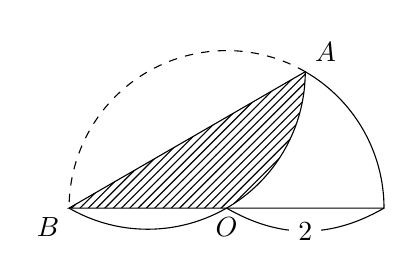
\begin{tikzpicture}
		\coordinate (O) at (0,0);
		\draw (-2,0) coordinate (B) -- (2,0) arc [start angle=0, delta angle=60, radius=2] coordinate (A) --cycle;
		\draw[dashed] (A) arc [start angle=60, end angle=180, radius=2];
		\draw (-2,0) arc [start angle=240, delta angle=120, radius=2];
		\fill[pattern=north east lines] (B) -- (O) arc [start angle=300, end angle=360, radius=2] -- cycle;
		\node[below] at (O) {$O$};
		\node[below left] at (B) {$B$};
		\node[above right] at (A) {$A$};
		\draw (O) to[bend right] node [fill=white, midway] {$2$} (2,0);
	\end{tikzpicture}
	\caption{}
\end{figure}

半径$2$の半円板を,$B$を通るような直線で,円周が中心$O$を通るように折り返す.このとき,折り返した部分と元の半円板が重なる領域の面積を考える(図\ref{fig:blue1}斜線部).

答えは
\[
	4\pi\cdot\dfrac16=\frac23\pi
\]
である.実際,折り返した部分を元に戻し,その上で$B$を$O$にずらせば,求める面積がもとの半円板の面積の$1/3$であることが分かる.解説の図は打つのが面倒なのでいつか追加することにする.

\subsection{パイの分割}

あるパイを100人に順番に,$n$人目はその時点での残りの$n$\%を得るように取り分ける.このとき,一番多くのパイを得るのは何人目かを考えよう.

$n$人目が得るパイが全体に占める割合を$\pi_n$とおく.$n-1$人目が取り分ける前に残っているパイが全体に占める割合は$(100/(n-1))\pi_{n-1}$と表せるので,$\pi_n$は
\[
	\pi_n=\frac n{100}\left(\frac{100}{n-1}\pi_{n-1}-\pi_{n-1}\right)\quad (2\le n\le100)
\]
を満たすと分かる.
よって
\[
	\frac{\pi_n}{\pi_{n-1}}=\frac{n(100-n+1)}{100(n-1)}
\]
なので, 
\begin{align*}
	\pi_n\ge \pi_{n-1}\quad\Longleftrightarrow\quad (n-1)n\le100
\end{align*}
を得る.
$n=10$はこの不等式を満たすが$n=11$は満たさないので,$\pi_n$は
\[
	\pi_1<\pi_2<\dotsb<\pi_9<\pi_{10}>\pi_{11}>\dotsb>\pi_{100}
\]
を満たす.従って,一番多くパイを得るのは10人目である.

\subsection{積分問題}

\[
	\int_1^\infty \frac{2x\{x\}-\{x\}^2}{x^2[x]^2} \,dx
\]
を考える.ただし,$\{x\}$は$x$の小数部分を表す.

$x=[x]+\{x\}$であることから,
\begin{align*}
	\int_1^\infty \frac{2x\{x\}-\{x\}^2}{x^2[x]^2} \,dx &= \int_1^\infty \frac{\{x\}(x+(x-\{x\}))}{x^2[x]^2} \,dx \\
	&= \int_1^\infty \frac{(x-[x])(x+[x])}{x^2[x]^2} \,dx \\
	&= \int_1^\infty \frac{x^2-[x]^2}{x^2[x]^2} \,dx \\
	&= \int_1^\infty \left( \frac1{[x]^2}-\frac1{x^2}\right) \,dx
\end{align*}
を得る.
\begin{align*}
	&\begin{aligned}
		\int_1^\infty \frac1{[x]^2}\,dx &=\lim_{R\to \infty} \left( \sum_{n=1}^{[R]-1} \int_n^{n+1} \frac1{[x]^2} \,dx + \int_{[R]}^R \frac1{[x]^2}\,dx\right) \\
		&=\lim_{R\to\infty} \left( \sum_{n=1}^{[R]-1} \int_n^{n+1} \frac1{n^2} \,dx + \int_{[R]}^R \frac1{[R]^2} \right) \\
		&=\lim_{R\to \infty} \left( \sum_{n=1}^{[R]-1} \frac1{n^2} + \frac{R-[R]}{[R]^2} \right)\\
		&=\frac{\pi^2}6,
	\end{aligned} \\
	\\
	&\int_1^\infty \frac1{x^2}\,dx = \left[ -\frac1x \right]_1^\infty=1
\end{align*}
より,
\[
	\int_1^\infty \frac{2x\{x\}-\{x\}^2}{x^2[x]^2} \,dx  \int_1^\infty \left( \frac1{[x]^2}-\frac1{x^2}\right) \,dx=\frac{\pi^2}6-1.
\]

\subsection{自然変換の簡単な例}

$G,H$は群,$\arrow{f,g}GH$は群準同型写像とする.$G,H$は1つの対象からなる圏と見なせて,このとき$f,g$は$G$から$H$への関手となる.このとき,自然変換$\nat{\tau}fg$を考える.
\[
	\begin{tikzcd}
		G \ar[r, "f", bend left=50, ""{name=f, below}] \ar[r, "g"{below}, bend right=50, ""{name=g}] & H
		\ar["\tau", Rightarrow, from=f, to=g]
	\end{tikzcd}
\]
自然変換の定義により,$\tau$は$H$の元であり,任意の元$x\in G$に対して
\[
	g(x)\tau=\tau f(x)
\]
が成り立つ.つまり,$g(x)=\tau f(x)\tau^{-1}$が成り立つことが,$\tau$が$f$から$g$への自然変換となる必要十分条件である.例えば,単位元$e$は自然変換となる.これは,2つの準同型$f,g$が操作の変換として本質的に同じであると言っている:$f$を作用させることと$g$を作用させることは,$H$の元(操作)によって移りあえるのである.

\section{その他}

有象無象にメモした,もしくは頭の中にあるだけだった考えをここに書きます.

\subsection{TikZによる空間図形の描写}

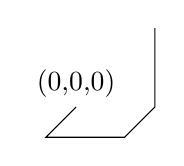
\begin{tikzpicture}
	\draw (0,0,0) node [above]  {(0,0,0)}--(0,0,1)--(1,0,1)--(1,0,0)--(1,1,0);
\end{tikzpicture}
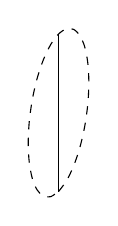
\begin{tikzpicture}
	\draw[style=dashed, domain=-pi:pi, variable=\t, smooth] plot(0,{cos(\t r)},{sin(\t r)});
	\draw (0,1,0)--(0,-1,0);
\end{tikzpicture}

空間内の媒介変数表示された関数をプロットできるとさらにうれしい.妥協策は,1つの成分の値を固定して2変数の媒介変数表示に持ち込んで,繰り返しプロットすることか:

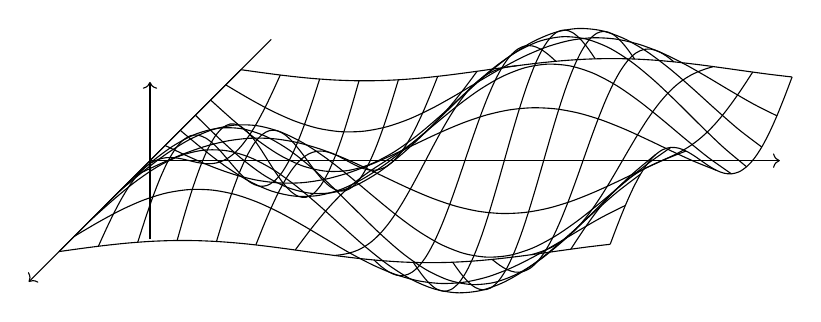
\begin{tikzpicture}
	\foreach \z in {-3,-2.5,...,3} {
		\draw[domain=0:7, variable=\x,smooth] plot(\x,{sin(\x r)*sin(\z r)},\z);
	}
	\foreach \x in {0,0.5,...,7} {
		\draw[domain=-3:3, variable=\z,smooth] plot(\x,{sin(\x r)*sin(\z r)},\z);
	}
	\draw[->] (0,0)--(8,0);
	\draw[->] (0,-1)--(0,1);
	\draw[->] (0,0,-4)--(0,0,4);
\end{tikzpicture}

コンパイルが重い!\texttt{\textbackslash addplot3}とかいうコマンドで何とかなるらしい.

\subsection{\ref{subsec:reciprocal}再考}\label{subsec:Re:reciprocal}

\S\ref{subsec:reciprocal}で現れた方程式(\ref{eq:recip})について,$a+b=x$,$a-b=y$とすれば
\begin{equation}\label{eq:recipxy}
	y=x^n
\end{equation}
のように表せる.このとき$a=\dfrac{x+y}2$,$b=\dfrac{x-y}2$であるから,方程式(\ref{eq:recip})の解を調べるには(\ref{eq:recipxy})を調べれば十分である.

\S\ref{subsec:reciprocal}と同様に,$n=-2$の場合について考えてみる.$x^2=\dfrac1y$より,$y>0$を1つ定めれば$x=\pm\dfrac1{\sqrt y}$を得るので,このときのすべての$(a,b)$は
\[
	\begin{dcases}
		a=\frac12\left(t\pm\frac1{\sqrt t}\right),\\
		b=\frac12\left(-t\pm\frac1{\sqrt t}\right)
	\end{dcases}
	\quad(t>0)
\]
で表せる.

ところで,\S\ref{subsec:reciprocal}では$a$を固定して解を求めた.これは(\ref{eq:recipxy})のグラフと$y=-x+2a$のグラフの交点を求めることに他ならない;$x=a+b$を$b$について解き,それを$y=a-b$に代入すればよい.この考え方から,$a$に対して唯一つの$b$が定まるような$a$の範囲を得ることができる.

\begin{figure}[ht]\label{fig:recip}
	\centering
	\begin{tikzpicture}
		\draw[->] (-3,0)--(3,0) node[below] {$x$};
		\draw[->] (0,-2)--(0,4) node[left] {$y$};
		\begin{scope}
			\clip (-3,-2) rectangle (3,4);
			\draw[domain=-3:-0.1, smooth] plot(\x, {1/((\x)^2)+\x});
			\draw[domain=0.1:3, smooth] plot(\x, {1/(\x^2)+\x});
			\draw[dashed] plot(\x,\x);
		\end{scope}
		\draw[dashed] (-2,3) node[left] {$\dfrac32 \sqrt[3]2$} to[bend left] (0,{3/2*2^(1/3)}) coordinate (p) --  ({2^(1/3)},{3/2*2^(1/3)}) -- ({2^(1/3)},0) node[below] {$\sqrt[3]2$};
		\fill (p) circle (1.5pt);
	\end{tikzpicture}
	\caption{$y=\dfrac1{x^2}+x$のグラフ}
\end{figure}

$f(x)=\dfrac1{x^2}+x$とおく.$y=f(x)$と$y=2a$のグラフが1点のみで交わるような$a$の範囲が求めたいものである.$y=f(x)$のグラフは図\ref{fig:recip}に示した通りであるから,求める範囲は$2a<\dfrac32 \sqrt[3]2$を解いて
\[
	a<\dfrac34 \sqrt[3]2
\]
となる.$a$の最小値が存在しないことは$f(x)$の連続性と$\lim_{x\to-\infty}f(x)=-\infty$などから分かる.

以上では$n=-2$の場合に限定して考えたが,同様にして他の整数$n$に対して$(a,b)$を調べることができるだろう.

\subsection{正規部分群について}

$G$を群,$H$をその部分群とする.普通,$G$の$H$による剰余群$G/H$は$H$が正規部分群,つまり任意の$g\in G$に対して$gH=Hg$が成り立つときに定義される.直感的には
\[
	(xH)(yH)=xHyH=xyHH=(xy)H
\]
と計算するために要請される条件であるが,
\begin{equation}\label{eq:xHyH}
	(xH)(yH)=zH
\end{equation}
となるような$z$の定め方は他に存在しないのか.

松坂和夫『代数系入門』の演習問題にその答えがある:
\begin{quote}
	11. $H$を$G$の部分群とし,$H$を法とする任意の2つの左剰余類の積は$H$を法とする1つの左剰余類になるとする.そのとき$H$は$G$の正規部分群であることを示せ.~\cite[p.65]{松坂}
\end{quote}
つまり,$G/H$が積により群となるための必要条件(従って必要十分条件)が,$H$が$G$の正規部分群であることだと主張している.

\begin{proof}
	任意に$x\in G$を取る.仮定より,$(xH)(x^{-1}H)=yH$となる$y\in G$が存在する.ここで,$H$が群であることから,$G$の単位元$1$は$H$に含まれるので,ある$h'\in H$が存在して
	\[
		1=x1x^{-1}1=yh'
	\]
	を満たす.よって$y=h'^{-1}\in H$であるから,結局$yH=H$が従う.従って,$(xH)(x^{-1}H)=H$だから,任意の$h\in H$に対して$xhx^{-1}=xhx^{-1}1\in H$となる.よって$H$は$G$の正規部分群である.
\end{proof}

従って,$G$の積が$G/H$上でwell-definedになるには$H$が$G$の正規部分群であることが必要であり,そのとき(\ref{eq:xHyH})における$z$は$z\equiv xy\ (H)$を満たさざるを得ない.

\subsection{有限集合の間の写像について}

$X,Y$を集合,$\arrow{f}XY$を写像とする.$|X|=|Y|$としよう.このとき,$f$が単射であることと全単射であることは同値である.実際,$f(X)\subset Y$であり,単射性から$f(X)$の元はすべて相異なるので$|f(X)|=|X|=|Y|$である.従って,定理\ref{prop:set_eq}により$f(X)=Y$を得るので,$f$は全射であり,従って全単射となる.逆は全単射の定義により明らかである.

これは,有限集合の圏$\cat{Set}_f$において,射$f$がモニックであることとエピであることが同値であると換言できる.

\begin{thebibliography}{9}
\bibitem{松坂} 松坂和夫,『代数系入門』,岩波書店,1976年,第1版
\end{thebibliography}


\end{document}